\documentclass[a4paper,11pt,article]{memoir}

%%%%%%%%%%%%%%%%%%%%%%%%%%%%%%%%%%%%%%%%%%
% Fonts
\usepackage[T1]{fontenc}
\usepackage[utf8]{inputenc}
\usepackage[francais]{babel}
\usepackage{microtype}
\usepackage{lmodern}

\usepackage[scaled=0.95]{helvet}
\renewcommand\familydefault{\sfdefault}
\usepackage[EULERGREEK]{sansmath}\sansmath % sans-serif math w/ greeks

%%%%%%%%%%%%%%%%%%%%%%%%%%%%%%%%%%%%%%%%%%
% Page layout

\usepackage[margin=2cm]{geometry}
\pagestyle{plain}
\setlength{\parindent}{0pt}

\renewcommand*{\chaptitlefont}{\secheadstyle}% for toc, bib, and friends 
\setsecheadstyle{\Large} % default: \Large\bfseries
\setsubsecheadstyle{\large} % default: \Large\bfseries
\setsecnumdepth{subsubsection}
\settocdepth{subsubsection}
\renewcommand*{\thesection}{\arabic{section}}
\renewcommand*{\thesubsection}{\thesection.\arabic{subsection}}
\setbeforesecskip{3 ex plus 1ex minus 1ex} % default(ex): 3.5+1-.2
\setaftersecskip{2 ex plus 1ex minus 1ex} % default(ex): 2.3+.2
\setbeforeparaskip{2 ex plus 1ex minus 1ex}% default(ex): 3.25+1-.2

\setcounter{secnumdepth}{3}

\renewcommand\title[1]{{\LARGE\fontfamily{pag}\selectfont #1}\par\bigskip}

%%%%%%%%%%%%%%%%%%%%%%%%%%%%%%%%%%%%%%%%%%%
% Utilities


% \usepackage{minted} % syntax coloring % If you don't have the
% 'minted' package, just turn all listings to verbatim :-)

\usepackage{boxedminipage}

\newenvironment{reponse}{
\begin{center}
  \begin{boxedminipage}{0.9\linewidth}\underline{Réponse}~:~
}{
  \end{boxedminipage}
\end{center}
}

\usepackage{graphicx}


%%%%%%%%%%%%%%%%%%%%%%%%%%%%%%%%%%%%%%%%%%%
% Document body

\begin{document}

\includegraphics[height=2cm]{fig/insa.pdf}
%
\hfill
%
{\fontfamily{pag}\selectfont Département IF / Architecture Matérielle}

\bigskip

\title{TP2: Développement Croisé}

\bigskip
\noindent\par\parbox{.48\textwidth}{Nom : Bertron} \parbox{.48\textwidth}{Prénom : Aurélien}
\bigskip
\noindent\par\parbox{.48\textwidth}{Nom : Losbar} \parbox{.48\textwidth}{Prénom : Thomas}
\bigskip
\noindent\par\parbox{.2\textwidth}{Groupe : 2} \parbox{.2\textwidth}{Binôme : B3229}

\bigskip

\paragraph{Question 1 ---}  La fonction \verb|lcd_init()| écrit dans les registres LCDACTL, LCDAPCTL (0 et 1) et LCDMEM (1 à 20).

\paragraph{Question 2 ---}  

\paragraph{Question 3 ---}  D'après MSP430.pdf[750], tous les registres font 8 bits. D'après datasheet.pdf[16], les registres 8 bits de périphériques sont situés entre les adresses 0FFh et 010h.

\paragraph{Question 4 ---}  Les plages d'adresses sont spécifiées à la même adresse :
%\begin{figure}
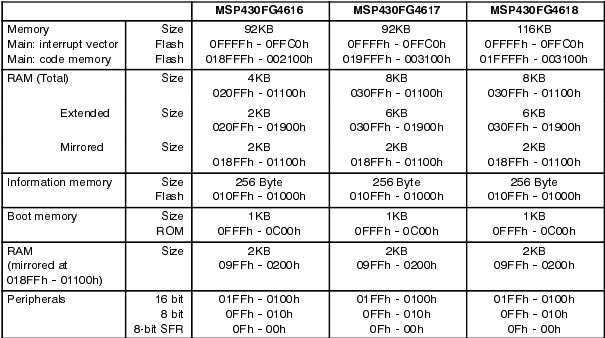
\includegraphics[height=6cm]{fig/plagesAdressage.png}
%\end{figure}

\paragraph{Question 5 ---}  Dans Compiler.pdf[207], on peut voir qu'en C, l'opérateur @ permet de définir l'adresse à laquelle est stockée une variable. Ces deux lignes sont des déclarations de macros qui permettent de définir une variable à une adresse donnée. La seule différence est la taille de la zone mémoire : 16 bits pour DEFW, 8 bits pour DEFC.

\paragraph{Question 6 ---}  Trouvé dans MSP430.pdf[750/736] : on voit que \(f_{LCD} = 2 \times mux \times f_{frame}\), on cherche $f_{frame}$. On indique dans le code que l'on divise ACLK par 512 (bits 5,6 et 7 de LCDACTL à 1). $f_{LCD}$ est donc égal à 32768 / 512 = 75,71 Hz. Donc $f_{frame} = f_{LCD} / (2 * 4) = 9,46Hz$, car mux = 4.

\paragraph{Question 7 ---}  Il nous faut changer les 3 derniers bits de LCDACTL. C'est à ça que sert la ligne 21 "(n<<5)", c'est à dire écrire n à partir du 5ème bit dans LCDACTL. Au lien de diviser ACLK par 512, on choisit de diviser par 128, ce qui donne une valeur pour $f_{frame}$ de 32 Hz. L'écran ne scintille plus.

\paragraph{Question 8 ---}  A la ligne LCDMEM[j] = 0xFF, on change 0xFF par 0 pour éteindre tous les segments.

\paragraph{Question 9 ---}  Le boîtier de l'écran possède 26 broches. LCD.pdf[3] nous montre qu'il y a 4 broches communes et 22 segments pins.

\paragraph{Question 10 ---}  22 * 4 = 88, il y a donc en tout 88 segments sur l'écran.

\paragraph{Question 11 ---}  Selon LCD.pdf[3], Dollar correspond à COM0 (P18) et à P26.

\paragraph{Question 12 ---}  Selon CPU.pdf[19], la pin 26 de l'écran est reliée à la pin 37 du MSP430. COM0 est reliée à la pin 52 du MSP430.

\paragraph{Question 13 ---}  Insérer code...

\paragraph{Question 14 ---}  Insérer code...

\paragraph{Question 15 ---}
\begin{verbatim}
// D'après Compiler.pdf[119], on met les 4 premiers paramètres de la fonction dans R12:R15, et le reste dans la pile
// Cela est possible car chaque paramètre est codé sur 16 bits, alors il y a un registre par paramètre. Si les paramètres étaient plus larges, il faudrait deux registres par paramètre, et donc plus de paramètres dans la pile.
0031E6    1230 0007          push.w  #0x7 // on ajoute le paramètre dans la pile
0031EA    1230 0006          push.w  #0x6
0031EE    1230 0005          push.w  #0x5
0031F2    422F               mov.w   #0x4,R15 // on ajoute le paramètre dans un registre
0031F4    403E 0003          mov.w   #0x3,R14
0031F8    432D               mov.w   #0x2,R13
0031FA    431C               mov.w   #0x1,R12
0031FC    12B0 3182          call    #lcd_display_seven_digits // on appelle la sub-routine
\end{verbatim}

\paragraph{Question 17 ---}

\paragraph{Question 18 ---}  Selon Compiler.pdf[196], n est un entier non signé, codé sur 16 bits.

\paragraph{Question 19 ---}  On n'utilise ici que des variables codées sur 16 bits. Le résultat attendu de la multiplication de 30 000 par 40 000 est 1 200 000 000 or, la valeur maximum codable sur 16 bits est 65 535, il y a donc un dépassement de capacité.

\paragraph{Question 20 ---}  Le résultat de cette multiplication est codable sur 32 bits (valeur maximum : 4 294 967 295), on peut donc utiliser un \verb|unsigned long| (toujours selon Compiler.pdf[196])

\paragraph{Question 21 ---}  En remplacant au moins l'un des opérandes en \verb|unsigned long| pour le coder sur 32 bits, la valeur calculée est correcte. Il est intéressant de voir comment le compilateur gère ces grands nombres en les stockant dans deux registres 16 bits, et en effectuant de ce fait beaucoup plus d'opérations (copies, effacements, etc.)

\paragraph{Question 22 ---}  On choisit d'utiliser le type \verb|uint16_t| pour n afin d'avoir des valeurs assez grandes, mais on peut noter que le choix du type permet également de choisir la valeur maximale du tirage au sort : 65535 pour \verb|uint16_t| et 255 pour \verb|uint8_t|.

\paragraph{Question 23 ---}  Lorsqu'on veut faire une multiplication par un petit nombre, le compilateur s'arrange pour simplifier la multiplication, c'est à dire éviter de faire plusieurs add à la suite. On le voit dans ce code lors d'une multiplication par 3 :

\begin{verbatim}
alea:
 003246    421F 1100          mov.w   &n,R15 # Récupération de la variable en zone statique
 00324A    4F0E               mov.w   R15,R14
 00324C    5F0F               rla.w   R15 # Rotation à gauche : multiplication par deux
 00324E    5E0F               add.w   R14,R15 # on ajoute encore n à lui-même => multiplication par 3
 003250    503F 0005          add.w   #0x5,R15 # on ajoute encore 5 à n
 003254    4F82 1100          mov.w   R15,&n # et on stocke la nouvelle valeur de n en zone statique
\end{verbatim}



\end{document}
